\documentclass{these}
\usepackage[utf8]{inputenc} %spécification de l'encodage du fichier .tex, à 
                            %changer si c'est du latin1
\usepackage[french]{babel}
\usepackage[T1]{fontenc}
\usepackage{cite}     % pour les citations multiples
\usepackage{amsthm}
\usepackage{graphicx}
 \usepackage{float}
 \usepackage[linesnumbered, french,onelanguage,vlined,ruled]{algorithm2e}
 
 \usepackage{fontspec}
\usepackage[usenames,dvipsnames]{pstricks}
 \usepackage{epsfig}
 \usepackage{pst-grad} % For gradients
 \usepackage{pst-plot} % For axes
 \usepackage[space]{grffile} % For spaces in paths
 \usepackage{etoolbox} % For spaces in paths
 \makeatletter % For spaces in paths
 \patchcmd\Gread@eps{\@inputcheck#1 }{\@inputcheck"#1"\relax}{}{}
 \makeatother 
 
 
 
\theoremstyle{definition}
\newtheorem{theorem}{Théorème}[section]
\newtheorem{definition}{Définition}[section]
\newtheorem{lemme}{Lemme}[section]
\newtheorem{preuve}{Preuve}[section]
\newtheorem{exemple}{Exemple}[subsection]

\title{Algorithmique de graphes pour l'aide à la décision dans la construction moléculaire }
\author{Stéfi NOULEHO ILEMO}
\date{XX - mois - XXXX}
\labo{DAVID}
\school{EDSTIC}
\speciality{Informatique}
\university{l'Université de Paris-Saclay}{UNIVERSITÉ DE PARIS-SACLAY}
%\ISBN{} %à remplir et décommenter lorsque ce numéro est connu.
\advisor[M]{Dominique BARTH} %Directeur de thèse
\coadvisor[M]{Marc-Antoine WEISSER} %Co-directeur de thèse, si nécessaire
\jury{  %définition des membres du jury
\jurymember[M]{Z}{Président du jury}\\
\jurymember[M]{U}{Rapporteur}\\
\jurymember[M]{V}{Rapporteur}\\
\jurymember[M]{W}{Examinateur}\\
\juryadvisor\\    % inclut le directeur de thèse dans le jury
\jurycoadvisor    % inclut le co-directeur de thèse dans le jury, si nécessaire
}

\bibliographystyle{plain}
\begin{document}
\frontmatter
\maketitle

\resume{
%La commande preamble définit un chapitre de préambule (pas de
%numérotation, et apparait en plus petit dans la table des matières).

}

{
%La commande preamblenodoublepage définit un préambule qui ne commence pas
%nécessairement sur une page de droite. Elle est utile ici, afin que la version
%anglaise du résumé soit au verso de la version française.



}
%\input{remerciements.tex}
\tableofcontents

\mainmatter
\chapter*{Introduction}
Bla bla bla.
\chapter{Présentation détaillée du sujet}
\label{chap1}
\section{Titre de la premiere section}
Bla bla bla.
\section{Titre de la seconde section}
Re-bla bla bla.
Une citation \cite{bregier2004mas}.

\section{Conclusion}
Conclusion du chapitre.
\chapter{État de l'art sur la similarité moléculaire}
\label{chap2}

La similarité moléculaire joue un rôle important dans de nombreux aspects de la chémo-informatique tels que la recherche de similarité, la classification de bases de données moléculaires, la découverte de médicaments et l'analyse de la diversité moléculaire. La similarité englobe les positions atomiques, les conformations, la forme et la disposition spatiale des propriétés moléculaires\cite{dean2012molecular}. 

Cependant, la similarité entre deux molécules doit être optimisée par rapport aux applications examinées. C'est un domaine large et en constante évolution. Il existe de multiples mesures de similarité décomposés entre autre en ceux qui sont basés sur le graphe moléculaire, ceux qui basés de la conformation et ceux qui demandent un calcul de la fonction d'onde moléculaire. On distingue: 

\begin{itemize}
\item Les \textbf{mesures unidimensionnelles}\cite{dixon2001one} sont basées sur les propriétés physico-chimiques des molécules telles que le volume, la polarisation et le poids. Puisqu'elles ne prennent pas en considération les informations géométriques de la molécules, ces mesures sont généralement utilisés pour le clustering des bases de données\cite{downs1994similarity}.

\item Les \textbf{mesures $2D$} sont basées sur le graphe moléculaire. La mesure la plus répandue pour comparer les structures chimiques représentées en utilisant les empreintes est le coefficient de Tanimoto \cite{bajusz2015tanimoto}. La recherche de sous-structure via la sous-structure commune maximum (en anglais, Maximum Common Subgraph MCS\cite{rascal} se classe aussi dans cette catégorie.

\item Les  \textbf{mesures 3D} tel que l'empreinte $3D$ utilisent l'alignement des molécules dans l'espace. Contrairement aux méthodes $1D$ et $2D$, elles tiennent compte de la taille et de la forme des structures moléculaires (propriétés conformationnelles) \cite{shin2015three}.
Cependant, elles restent moins utilisées car beaucoup plus complexes\cite{bero2017similarity, barbosa}.

%empreintes 3D : pharmacophore fingerprints
\end{itemize}
La similarité que nous recherchons durant la thèse se situe sur la partie structurelle notamment les mesures $2D$ sur les graphes moléculaires. Dans la section \ref{tanimoto}, nous présenterons le quelques mesures de similarité basés sur le calcul d'empreintes dans le graphe moléculaire, plus précisement le coefficient de Tanimoto. Ensuite dans la Section \ref{mces}, nous exposerons la mesure de similarité basée sur le problème Maximum Common Edge Subgraph. 
%suites binaires = empreintes

%Dans ce chapitre, nous allons présenter quelques mesures de similarité

Ce chapitre contient également dans la Section \ref{theoriegraphe}, les définitions préliminaires sur les notions de cycles, bases de cycles, union de bases de cycles dans les graphes. Ces notions de la théorie de graphes seront utilisés dans les chapitres suivants. 


\section{Les mesures de similarité basés sur les empreintes}
\label{tanimoto}

Les empreintes ou suites binaires sont calculées à partir de la présence ou de l'absence de caractéristiques moléculaires. Elles sont généralement comparées en utilisant un coefficient de similarité en tant que mesure de la similarité entre les structures. %Cette méthode est particulièrement efficace dans le cas où les motifs sont faciles à calculer.

Pour calculer la similarité il faut dans un premier temps associer à chaque molécule, une empreinte. Dans un second temps choisir le coefficient adapté pour obtenir une mesure. 

\subsection{Le calcul des empreintes}

Les principales types d'empreintes sont les empreintes basées sur les notions de sous-structures, les empreintes topologiques ou basées sur le chemin, et les empreintes circulaires.


\begin{itemize}
\item Les empreintes basées sur des motifs (sous- structures) définissent les bits l'empreinte en fonction de la présence dans le composé de certaines sous-structures ou caractéristiques d'une liste donnée de motifs. Ces empreintes sont intéressantes lorsqu'elles sont utilisées avec des molécules susceptibles d'être recouvertes par la liste de motifs choisie. Elles le sont moins lorsque les molécules contiennent d'autres motifs, car leurs présence ne seraient pas représentés. Leur nombre de bits de l'empreinte est déterminé par le nombre de motifs, et chaque bit renseigne sur la présence ou à l'absence d'une caractéristique donnée dans la molécule. %Les motifs sont généralement 

\item Les empreintes topologiques analysent tous les fragments de la molécule en parcourant un chemin linéaire jusqu’à un certain nombre de liaisons, puis en hachant chacun de ces chemins pour créer l’empreinte. Ainsi toute molécule peut produire une empreinte digitale cohérente et sa longueur peut être ajustée. Ce type d'empreintes est utilisé pour la recherche de sous-structures. L’empreinte la plus connu sous le nom de Daylight \cite{} comporte jusqu'à 2048 bits et code toutes les motifs possibles à travers une molécule jusqu'à une longueur donnée.

\item Les empreintes circulaires ressemblent aux empreintes topologiques à la différence qu'au lieu de rechercher des chemins dans le graphe moléculaire, ils stockent l'environnement de chaque atome jusqu'à un rayon fixé. On distingue parmis les empreintes cirulaires : Extended-Connectivity Fingerprint (ECFP diamètre $4$ et $6$) basé sur l'algorithme de Morgan, Functional-Class Fingerprints (FCFP $4$ et $6$) et Molprint2D.

\end{itemize}
\subsection{Coefficients de similarité}
Les mesures de similarité suivantes supposent que deux empreintes avec de nombreux bits en commun sont similaires. Ce sont des mesures brutes mais étonnamment efficaces pour une large gamme d'applications.

En effet, l'information de présence ou d'absence d'un motif est moins exhaustive que le nombre d'occurrences de celui-ci, ce qui, à son tour, ne donne aucune information sur la façon dont les motifs survenus sont répartis dans la molécule. %Les descripteurs 2D ou topologiques capturent les informations relatives à la connectivité moléculaire, caractérisant formellement le graphe représentant le schéma de connexion interatomique dans la molécule. 

Le tableau \ref{tableauempreintes} présente les différentes mesures et distances connues pour obtenir un coefficient de similarité. La plus utilisée est le coefficient de Tanimoto qui consiste à faire le ratio entre le nombre de bits communs à $1$ et le nombbre total de bits à $1$ dans les deux empreintes. Ce coefficient est compris dans $[0,1]$ quelque soit la taille des empreintes. 

\begin{center}

\begin{table}[!ht]

\label{tableauempreintes}
\centering
\caption{
{\bf Coefficients de similarité et distance basés sur les empreintes}}
\begin{tabular}{|c|c|c|}
%\caption{\textbf{Coefficients de similarité et distance basés sur les empreintes}.   }
\hline
\textbf{Mesure de similarité }& \textbf{Intervalle} & \textbf{Formule} \\
\hline
\textbf{Similarité de Cosine}& $[0,1]$ & $\frac{c}{\sqrt{a\times b}}$\\
\hline
\textbf{Coefficient de Tanimoto}& $[0,1]$ & $\frac{c}{\sqrt{a+ b - c}}$\\
\hline
\textbf{Coefficient de Dice }& $[0,1]$ & $\frac{2 \times c}{\sqrt{a+ b}}$\\
\hline
\textbf{Distance euclidienne}& $[0,N]$ & $\sqrt{a + b - 2 \times c}$\\
\hline
\textbf{Distance de Hamming}& $[0,N]$ & $a + b - 2 \times c$\\
\hline
\textbf{Coefficient de Forbes}& $[0,1]$ & $\frac{c \times m}{
a \times b }$\\
\hline
\textbf{Distance de Soergel }& $[0,1]$ & $\frac{a + b - 2 \times c}{\sqrt{a+ b - c}}$\\
\hline


\end{tabular}
\vspace*{0.4cm}

On considère deux empreintes moléculaires $A$ et $B$. On note $m$, le nombre total de bits dans $A$ et $B$; a, b et c représente respectivement le nombre de bits à $1$ dans $A$, le nombre de bits à $1$ dans $B$ et le nombre de bits à $1$ à la fois dans $A$ et $B$.

\end{table}
\end{center}

\textcolor{red}{exemple de calcul Tanimoto ?}


\section{Similarité basé sur le Maximum Common Edge Subgraph (MCES)}
\label{mces}
Dans cette section, nous allons présenter le calcul de similarité basé sur la recherche de sous-graphe commun ayant un nombre maximum d'arêtes. Toutefois nous nous limiterons à la définition de la mesure exacte et nous n'allons pas présenter les heuristiques[refs].

Soient deux graphes moléculaires $G_1=(V_1,E_1)$ et $G_2=(V_2,E_2)$. 

\begin{definition}
Un \textit{sous-graphe commun induit} $G_{1,2}$ de $G_1$ et $G_2$ est un graphe isomorphe à des sous-graphes induits de $G_1$ et $G_2$. Un graphe $G_{1,2}$ est un sous-graphe commun induit maximum (MCIS) s'il contient un nombre maximum de sommets dans $G_1$ et $G_2$. Un graphe $G_{1,2}$ est un sous-graphe commun ayant un nombre d'arêtes maximum (MCES) s'il contient un nombre maximum d'arêtes communs dans $G_1$ et $G_2$.
\end{definition}

Un MCIS et un MCES peuvent être des sous-graphes non connexes.
\begin{figure}[H]
\label{mcis-mces}

\caption{(a) Deux graphes $G_1$ et $G_2$, (b) en gras un MCIS et (c) en gras un MCES.}
\begin{center}
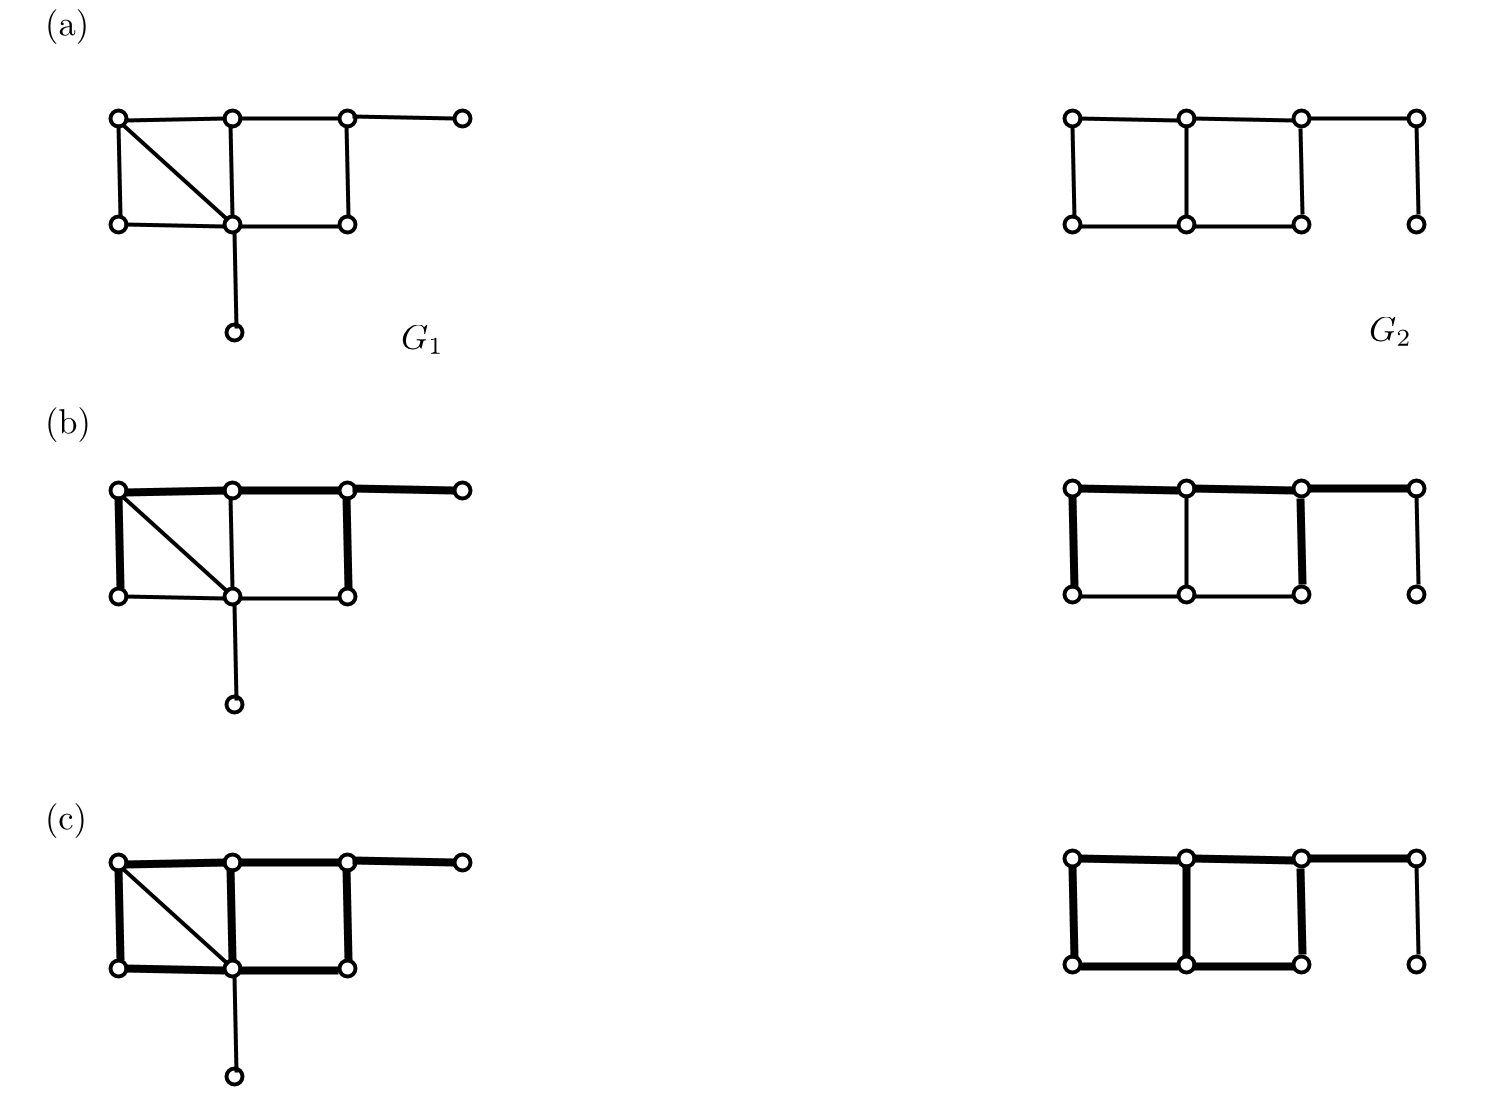
\includegraphics[scale=0.5]{mces_mcis.png}
\end{center}
\end{figure}

Pour le calcul de similarité trouver un sous-graphe commun ayant un nombre d'arêtes maximum  est pertinent \cite{rascal}. Dans la suite, on note $G_{1,2}=(V_{1,2},E_{1,2})$ un sous-graphe commun ayant un nombre maximum d'arêtes à la fois dans $G_1$ et $G_2$. La mesure de similarité $\mathrm{sim(G_{1},G_{2})}$ est :

\begin{eqnarray}
\mathrm{sim(G_{1},G_{2}) }= \frac{(|V _{12}| + |E _{12}| )^2 }{(|V _1| + |E_1| )\times (|V_2| + |E _2| )}
\label{eq:mces}
\end{eqnarray}

La recherche d'un sous-graphe commun ayant un nombre maximum d'arêtes se fait en trois étapes : le calcul du graphe produit, la recherche d'une clique maximum et l'extraction d'un sous-graphe commun à arêtes maximum entre $G_1$ et $G_2$.

\subsection{Le calcul du graphe moléculaire produit }

La première étape consiste à calculer le graphe moléculaire produit des linegraphes $G_1$ et de $G_2$ noté $L(G_1)\diamond (G_2)$. Le linegraphe $L(G_1)$ d'un graphe $G_1$ est un graphe dans lequel les arêtes de $G_1$ sont des sommets et deux sommets de $L(G_1)$ sont adjacents si et seulement si les arêtes correspondantes dans $G_1$ sont adjacentes.
Ce graphe moléculaire produit est telle que : $V(G_1\diamond G_2) = V(L(G_1)) \times V(L(G_2))$.

Soient deux sommets $(u_i,v_i), (u_j,v_j)  \in V(L(G_1)\diamond L(G_2))$. L'arête $[(u_i,v_i), (u_j,v_j)] \in E(L(G_1)\diamond L(G_2))$ si et seulement si :

\begin{itemize}
\item $(u_i,u_j) \in E(L(G_1))$, $(v_i,v_j) \in E(L(G_2))$ et $w(u_i,u_j)= w(v_i,v_j)$ \textbf{OU}
\item $(u_i,u_j) \notin E(L(G_1))$, $(v_i,v_j) \notin E(L(G_2))$.
\end{itemize}
La fonction $w(u_i,u_j)= w(v_i,v_j)$ vérifie la compatibilité entre les atomes et les liaisons. Elle associe les atomes et les liaisons du même type.

\begin{exemple}
On considère deux graphes moléculaires $G_1$ et $G_2$ de la Figure \ref{produit}(a). Les Figures  \ref{produit}(b) et \ref{produit}(c) montrent respectivement le calcul du linegraph des graphes  et les sommets du graphe produit.

\begin{figure}[H]
\label{produit}
\begin{center}
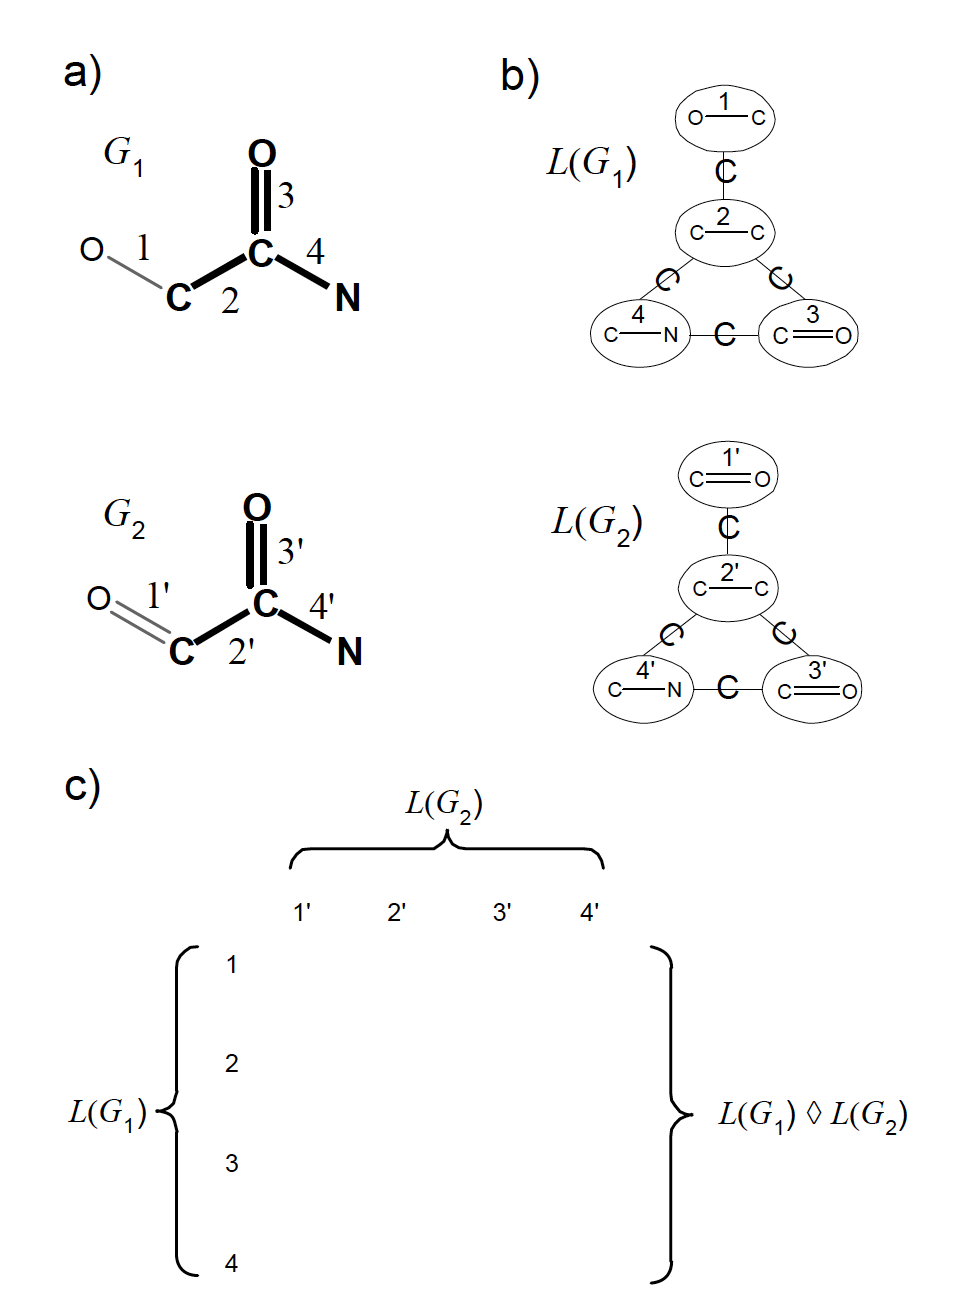
\includegraphics[scale=0.65]{produit.png}
\caption{Construction d'un graphe moléculaire produit}
\end{center}
\end{figure}
\end{exemple}

\subsection{La recherche d'une clique maximum et l'extraction d'un sous-graphe commun à arêtes maximum}

En utilisant le graphe produit des linegraphes de $G_1$ et $G_2$, on recherche une clique maximum à partir de laquelle on extrait un sous-graphe commun à arêtes maximum.

\begin{exemple}
En reprenant le graphe moléculaire produit de l'exemple précédent, on cherche une clique maximum.
\begin{table}[!ht]
\begin{flushleft}


\begin{tabular}{|p{1.0cm}|*{17}{@{\hskip.01mm}c@{\hskip.01mm}|}}
\hline
&$(1,1')$&$(1,2')$&$(1,3')$&$(1,4')$&$(2,1')$&$(2,2')$&$(2,3')$&$(2,4')$&$(3,1')$&$(3,2')$&$(3,3')$&$(3,4')$&$(4,1')$&$(4,2')$&$(4,3')$&$(4,4')$\\\hline
$(1,1')$&1&0&0&0&0&0&0&0&0&0&1&0&0&0&0&1\\ \hline
$(1,2')$&0&1&0&0&0&0&0&0&0&0&0&0&0&0&0&0\\ \hline
$(1,3')$&0&0&1&0&0&0&0&0&0&0&0&0&0&0&0&0\\ \hline
$(1,4')$&0&0&0&1&0&0&0&0&0&0&0&0&0&0&0&0\\ \hline
$(2,1')$&0&0&0&0&1&0&0&0&0&0&0&0&0&0&0&0\\ \hline
$(2,2')$&0&0&0&0&0&1&0&0&0&0&1&0&0&0&0&1\\ \hline
$(2,3')$&0&0&0&0&0&0&1&0&0&1&0&0&0&0&0&0\\ \hline
$(2,4')$&0&0&0&0&0&0&0&1&0&0&0&0&0&0&0&0\\ \hline
$(3,1')$&0&0&0&0&0&0&0&0&1&0&0&0&0&0&0&0\\ \hline
$(3,2')$&0&0&0&0&0&0&1&0&0&1&0&0&0&0&0&0\\ \hline
$(3,3')$&1&0&0&0&0&1&0&0&0&0&1&0&0&0&0&1\\ \hline
$(3,4')$&0&0&0&0&0&0&0&0&0&0&0&1&0&0&1&0\\ \hline
$(4,1')$&0&0&0&1&0&0&0&0&0&0&0&0&1&0&0&0\\ \hline
$(4,2')$&0&0&0&0&0&0&0&1&0&0&0&0&0&1&0&0\\ \hline
$(4,3')$&0&0&0&0&0&0&0&0&0&0&0&1&0&0&1&0\\ \hline
$(4,4')$&1&0&0&0&0&1&0&0&0&0&1&0&0&0&0&1\\ \hline

\end{tabular}
\end{flushleft}
\end{table}

On trouve une clique maximum de taille $3$. La taille de la clique est égale au cardinal de $E(G_{12})$. On fait ensuite une projection des arêtes de la clique dans $G_1$( ou $G_2$) pour obtenir un sous-graphe commun ayant un nombre maximum d'arêtes à la fois dans $G_1$ et $G_2$. Dans cet exemple, on a :
\begin{itemize}
\item $|V(G_1)| = 5$ et $|E(G_1)| = 4$
\item $|V(G_2)| = 5$ et $|E(G_2)| = 4$
\item $|V(G_{12})| = 4$ et $|E(G_{12})| = 3$


\end{itemize}
\begin{center}


 $\mathrm{sim(G_{1},G_{2}) }= \frac{(4 + 3 )^2 }{(5 + 4 )\times(5 + 4 )} = 0,6$
 \end{center}
\end{exemple}
La recherche de clique maximum est un problème NP-Complet. Il existe des heuristiques tels que les algorithmes de branch and bound \cite{rascal}.

\section{Quelques préliminaires de la théorie de graphes}
\label{theoriegraphe}
Dans cette section, nous allons définir quelques notions de la théorie de graphes \textcolor{red}{ (ref claude berges graph theory and application)} que nous utiliserons dans les chapitres suivants. Les informations sur les cycles constituent une partie importante de la topologie structurelle utilisée pour identifier et caractériser les structures moléculaires. Il est donc d’une importance cruciale d’obtenir ces informations pour diverses tâches en chimie computationnelle.

On considère un graphe simple et non orienté $G = (V, E)$ avec $n$ et $m$ respectivement le nombre de sommets et le nombre d 'arêtes de $G$. On note $V = \{v_1, v_2, ..., v_n\}$ avec $v_i$ le sommet d'indice $i$ et l'ensemble $E= \{e_1, e_2, ..., e_m\}$ tel que $e_j = [v_i, v_i']$.

\subsection{Chaînes et cycles}

\begin{definition}
Une chaîne est une suite fini d'arêtes consécutives $e_1, e_2, ...,e_k$ de $G$. La longueur d'une chaîne est le nombre d'arêtes qui la composent.
\end{definition}

Une chaîne est élémentaire si et seulement si elle passe au maximum une fois par chaque sommet. Une chaîne simple est une chaîne ne passant pas deux fois par une même arête.

\begin{definition}
Un cycle est une chaîne simple dont les extrémités sont identiques. Un cycle élémentaire ne contient pas d'autres cycles.
\end{definition}

Nous allons représenter un cycle élémentaire $c$ par un vecteur $v_c = (e_1^{c}, e_2^{c}, ...., e_m^{c})$ de taille $m$ avec $e_i^c = 1$ si et seulement si $e_i^c \in c$ et $e_i^c = 0$ sinon. La longueur d'un cycle notée $|c|$ vaut $\sum_{i = 1}^{m}e_i^c$.

\begin{exemple}
\label{exemplecycles}
Soit le graphe $G$ de la Figure \ref{chainescycles} avec $V = \{v_1, v_2, v_3, ...,v_9, v_{10}\}$ et $E = \{e_1, e_2, ...,e_{10}, e_{11}\}$. La chaîne $(e_1, e_2, e_3, e_4)$ est une chaîne élémentaire de $G$. Les cycles $c_1 =(e_1, e_2, e_{11}, e_8, e_9, e_{10})$ et $c_2 =(e_3, e_4, e_5, e_6, e_7,e_{11})$ sont des cycles élémentaires dont les vecteurs sont respectivement : 

\begin{center}
$v_{c_1} = (1, 1, 0, 0, 0, 0, 0, 1, 1, 1, 1)$\\
$v_{c_2} = (0, 0, 1, 1, 1, 1, 1, 0, 0, 0, 1)$

\end{center}
\begin{figure}[H]
\label{chainescycles}
\begin{center}
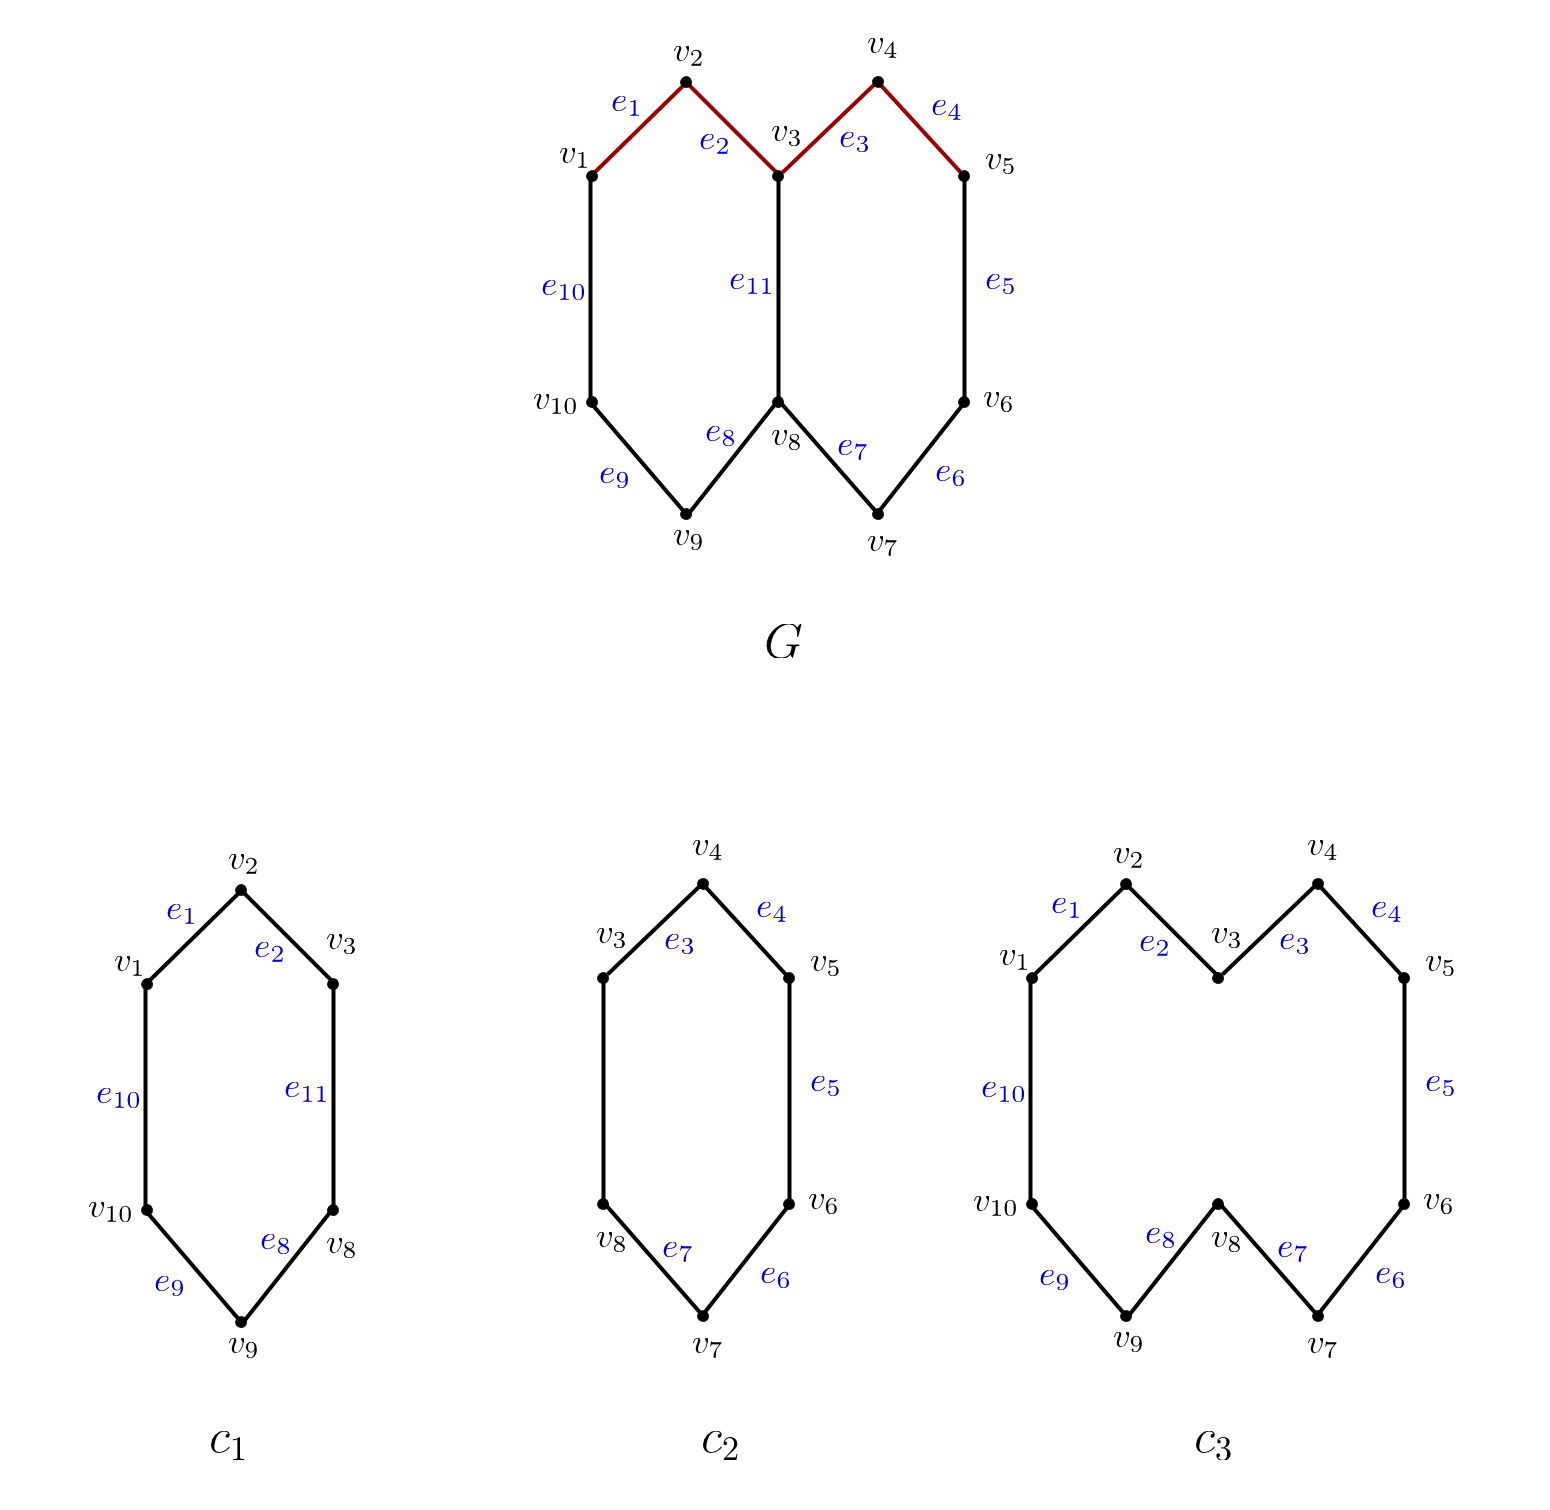
\includegraphics[scale=0.42]{chainescycles.png}
\end{center}
\caption{Chaînes et cycles élémentaires dans un graphe }
\end{figure}
\end{exemple}

On considère deux cycles élémentaires $c_1$ et $c_2$ dans un graphe $G$ telle que : $v_{c_1} = (e_1^{c_1}, e_2^{c_1}, ...., e_m^{c_1})$ et $v_{c_2} = (e_1^{c_2}, e_2^{c_2}, ...., e_m^{c_2})$.

\begin{definition}
L'union disjointe des cycles $c_1$ et $c_2$ notée $c_{12}$ est la différence symétrique des arêtes du graphe appartenant à $c_1$ et $c_2$. On note $c_{12} = c_1 \oplus c_2$ et le vecteur associé est $v_{c_{12}} = (e_1^{c_1} \oplus e_1^{c_2}, e_2^{c_1} \oplus e_2^{c_2}, ...., e_m^{c_1} \oplus e_m^{c_2})$.
\end{definition}

L'opérateur $\oplus$ représente le XOR binaire sur les $e_i^c$. L'union de deux cycles disjoints donne un vecteur composé de deux cycles disjoints. Dans l'Exemple \ref{exemplecycles}, le cycle $c_3$ est l'union disjointe des cycles $c_1$ et $c_2$.

%Le nombre cyclomatique
Lorsque dans un graphe, deux sommets d'un cycle sont reliés par une arête qui n'appartient pas au cycle, cette arête est appelée \textit{corde} du cycle. Un cycle de G dit induit lorsqu'il n'a pas de cordes.

\begin{definition}
Un cycle est dit \textbf{pertinent} s'il ne peut pas être obtenu par combinaison de cycles de longueur strictement plus petite.
\end{definition}

\subsection{Connexité et isthme}

\begin{definition}
Un graphe $G$ est \textbf{connexe} si toute paire de sommets $u,v \in V$ peut être reliée par une chaîne dans $G$.
\end{definition}
Un sous-graphe connexe maximal de $G$ est appelé composante connexe de $G$. Un graphe qui n'est connexe possède au moins $2$ composantes connexes.

%Un graphe connexe qui reste connexe après suppression de n’importe quel sous-ensemble de $k − 1$ sommets est dit $k-$connexe. 
Soit un graphe connexe $G$ et un ensemble d'arêtes $E'$ de $G$. Si le graphe $G -  E'$ n'est pas connexe, on dit que $E'$ est un séparateur de $G$. Si dans $G - E'$, deux sommets $u$ et $v$ sont dans deux composantes connexes différentes, on dit que $E'$ sépare $u$ de $v$ ou $E'$ est un $(u, v)-$séparateur.

\begin{definition}
 Pour $k \geq 1$, on dit que $G$ est $k-$connexe s'il a au moins $k+1$ sommets et aucun ensemble de $k -1$ sommets ne le sépare. Un graphe est k-arête-connexe, s'il a au moins deux sommets et aucun ensemble de $k - 1$ arêtes ne le sépare. 
\end{definition}

La valeur maximale $k$ pour laquelle une graphe G est $k - 1 $connexe est appelée connexité de $G$ et notée $\kappa(G)$. En particulier, lorsque $k = 2$ on parle de graphe $2-$connexe ou bi-connexe.
De même, la valeur maximale $k$ pour laquelle une graphe $G$ est $k-$arête-connexe est appelée arête-connexité de G et notée $\kappa′(G)$.

\begin{definition}
Une arête d'un graphe est un \textbf{isthme} si sa suppression augmente le nombre de composantes connexes du graphe. 
\end{definition}
Si le graphe est connexe, une arête est un isthme si et seulement si elle n'appartient à aucun cycle.

\subsection{Base de cycles}

Dans un graphe, on appele générateur de cycles $\zeta$, un ensemble fini de cycles tel que tout cycle de $G$ peut être obtenu par combinaison des cycles de $\zeta$.

\begin{definition}
On appelle une base de cycles $\mathcal{B}$, un ensemble de cycles linéairement indépendants et générateur.

\end{definition}

Soit $G$ un graphe de $n$ sommets, $m$ arêtes et $p$ composantes connexes,
la dimension d’une base de cycles est le nombre cyclomatique de $G: \nu(G)=m-n+p$. La longueur d'une base de cycles $\zeta$ est la somme des longueurs des cycles de la base. Il existe $2$ principales types de bases de cycles : les base de cycles fondamentales et les bases de cycles de longueurs minimum.

\subsubsection{Base de cycles fondamentale}

Lorsque le graphe $G$ est connexe, il est possible d'obtenir des bases de cycles en utilisant les arbres couvrants. Ces bases de cycles sont appelées \textbf{bases de cycles fondamentales} \cite{kir}.

Soit $T$ un abre couvrant arbitraire de $G$. Pour obtenir une base de cycles fondamentale, on rajoute à chaque fois à $T$, une arête de $G$ qui n'appartient pas à $T$. A chaque ajout, on cree un cycle qui appartient à la base de cycle fondamentale. On repète le procédé $m-n+1$ fois.

Cependant, trouver un abre couvrant tel que la base de cycles fondamentale soit minimum est un problème NP-Complet.

\subsubsection{Base de cycles de longueur minimum}

Une base de cycles de longueur minimum ou Mimimum Cycle Basis (MCB) est une base de cycles ayant une longueur minimale. Il existe plusieurs algorithmes pour trouver de telles bases. En chimie, les algorithmes developpés et applicables sur les structures moléculaires et graphes simples sont connus sous le nom de Smallest Set of Smallest Rings (SSSR)\cite{LeeJoon,Zamora,Qian}. En informatique, les algorithmes MCB d'une grande robustesse, sont concus pour des graphes en général \cite{horton,golynski2002polynomial,berger2004minimum,kavitha2004faster}.

Dans un graphe, il peut y avoir plusieurs bases de cycles de poids minimum. Lorsqu'il existe une unique base de cycles minimum $\mathcal{B}$ dans un graphe, cette base est aussi l'ensemble de cycles pertinents du graphe.

%\subsubsection{Ensembles de cycles pertinents}
\subsubsection{Union des bases de cycles de longueur minimum}


Également appelé ensemble de cycles pertinents, l'union des bases de cycles de longueur minimum est défini comme le plus petit ensemble canonique de cycles qui décrit la structure cyclique d'un graphe\cite{vismara}. Sa construction passe par l'obtention d'une représentation compacte servant de prototype pour les énumérer.
\chapter{Modèle de graphe de cycles}
\label{chap3}


Dans ce chapitre, nous allons définir formellement le modèle de graphes de cycles. Le graphe de cycles d'une molécule représente la partie structurelle de  celle-ci et est construit en utilisant son graphe moléculaire. Nous construisons ce modèle pour calculer la similarité structurelle entre molécules. Ainsi, il est primordial que des molécules structurellement similaires aient des graphes de cycles similaires. 

Cette représentation de la partie structurelle d'une molécule se fait à une échelle gros-grain. On ne se situe pas à l'échelle atomique comme dans les graphes moléculaires mais à l'échelle cyclique. L'élaboration de ce modèle gros-grain appelé par la suite graphe de cycles passe d'une part par la construction d'un ensemble de cycles pertinent pour décrire la structure moléculaire et d'autre part par l'interconnexion de ces cycles en fonction de leurs interactions dans la molécule. On souhaite garantir la notion de canonicité et la proximité sur les graphes de cycles.  La canonicité signifie que deux graphes moléculaires isomorphes et ayant une numérotation de sommets différente aient des graphes de cycles isomorphes. Elle garantie également qu'à un graphe moléculaire, on associe un unique graphe de cycles quelque soit la numérotation des sommets. La proximité quand à elle signifie que si deux graphes moléculaires sont proches (elles diffèrent d'un cycle par exemple) alors les graphes de cycles le seront aussi. De plus, pour le chimiste, certains "grands" cycles dans les molécules ne définissent pas la structure de celle-ci. Il s'avère donc nécessaire de ne pas sauvegarder une certaine taille de cycles dans les graphes de cycles.

Dans la section \ref{intuition}, nous présentons et analysons une construction intuitive du graphe de cycles d'une molécule. Ensuite, nous définissons dans la section \ref{interconnexion}, le graphe de cycles qui capture la structure de cycles et l'interconnexion de ces cycles. Plus particulièrement, nous expliquons comment relier les cycles dans le graphe de cycles en respectant la structure du graphe moléculaire. Finalement dans la Section \ref{generateurcycles} nous présenterons cette section l'algorithme permettant d'avoir une base de cycles pertinente et suffisante pour capturer la partie structurelle des molécules. Nous verrons la notion d'hiérarchie pour limiter la taille des cycles dans le graphe de cycles.

\section{Une représentation intuitive du graphe de cycles }
\label{intuition}

%Lorsqu'on parle du graphe cycles modélisant l'interconnexion des cycles dans une molécule, l'un des modèles que l'on peut construire intuitivement est tel que:  l'ensemble des sommets contient des cycles pertinents qui definissent de la structure de la molécule et 

On veut construire un graphe de cycles d'une molécule basé sur sa partie structurelle. Bien que le graphe moléculaire modélise globalement l'ensemble de l'information structurelle, il n'encode pas explicitement l'information cyclique. L'hypothèse étant que des molécules similaires sont structurellement similaires et que la partie structurelle d'une molécule est défini par l'interconnexion des cycles pertinants présentes dans celle-ci. 
Un \textit{cycle pertinent} est un cycle simple et élémentaire ne pouvant être obtenu par combinaison de cycles plus petits \cite{vismara}. 

Pour s'assurer que l'on capture les cycles pertinents, on pourrait au premier abord, prendre tous les cycles de la molécule. Cependant, compter tous les cycles dans un graphe est NP-complet sachant qu'il peut y avoir un nombre exponentiel. Pour son usage dans la mesure de similarité, la représentation du graphe de cycles  d'une molécule doit contenir un nombre minimal de cycles mais suffisant pour décrire au mieux sa structure ; il s'avère donc inutile de prendre tous les cycles de la molécule pour construire le graphe de cycles.

Une base de cycles d'un graphe quand elle contient un ensembe fini de cycles élémentaires (cf. chap2). Les cycles d'une base sont pertinents. Pour construire le graphe de cycles (Figure \ref{grapheintuitif}) d'une molécule $\mathcal{M}$, nous prenons intuitivement un hypergraphe $GC = (VC,EC,\mu)$ (défini par \cite{benoit}) :
\begin{itemize}
\item L'ensemble de sommets $VC$ est une base de cycles $ \mathcal{B}$. Chaque sommet $c$ correspond à un cycle pertinent et $\mu(c)$ correspond au sous-graphe moléculaire dans $\mathcal(M)$ contenant les atomes et liasons qui appartient au cycle $c$.
\item Deux cycles $c_1$ et $c_2$  de $VC$ sont reliés par une arête si et seulement si elles partagent au moins un atome dans le graphe moléculaire de $\mathcal{M}$ c'est à dire $\mu(c_1) \cap \mu(c_2) = \emptyset$. 
\end{itemize}  

\begin{figure}[H]
\label{grapheintuitif}

\begin{center}
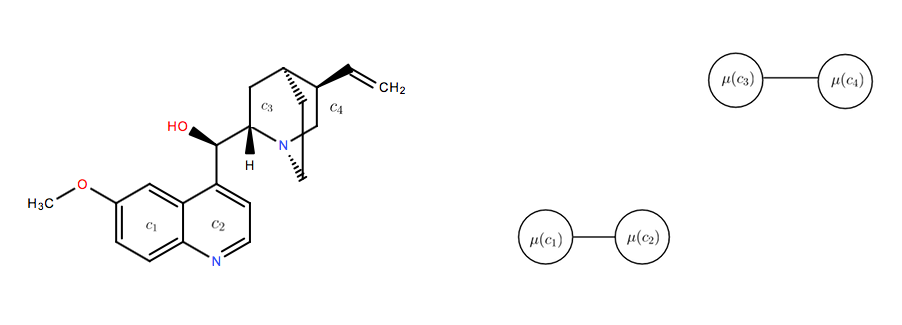
\includegraphics[scale=0.45]{exemple_intuitif_correct.png}
\end{center}
\caption{Graphe moléculaire de la quinine et le graphe de cycles intuitif associé}
\end{figure}

En observant le graphe de cycles de la Figure \ref{grapheintuitif}, on ne peut pas savoir exactement si le graphe moléculaire possède $2$ composantes connexes ou dans le contraire, sur quel cycle entre $c_1$ et $c_2$ les cycles $c_3$ et $c_4$ sont liées dans $\mathcal{M}$. Es-ce le cycle $c_3$ qui est relié au cycle $c_1$ ? ou au cycle $c_2$ ? ou à la fois à $c_1$ et $c_2$?

On pourrait tout à fait donner comme graphes moléculaires associés au graphe de cycles de la quinine, les graphes de la Figure \ref{exempleintuitif}.

\begin{figure}[H]
\label{exempleintuitif}

\begin{center}
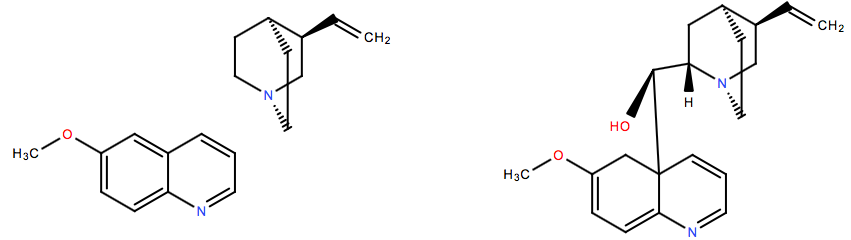
\includegraphics[scale=0.45]{exemple_graphes.png}
\end{center}
\caption{Graphes moléculaires ayant le même graphe de cycles que la quinine.}
\end{figure}

On constate dès lors que ce modèle n'est pas suffisant notamment :
\begin{itemize}
\item Au niveau de l'interconnexion des cycles: il semble logique que deux cycles ayant des atomes en commun soient liés dans $GC$ mais il faudrait aussi rajouter des liens supplementaires entre cycles indirectement liés pour réduire l'ambigüité et mieux décrire la structure des molécules.

\item Au niveau de la base de cycles : Elle n'est pas nécessairement unique ! Ce qui entrainerait dans la construction du graphe de cycles que l'on puisse avoir un graphe de cycles différent en fonction de la base choisi. En terme de similarité, cela reviendrait à dire qu'une molécule n'est pas totalement similaire à elle-même.
\end{itemize} 

\section{Interconnexion des cycles}
\label{interconnexion}
Nous avons vu dans la section précédente que le graphe de cycles devrait avoir suffisamment d'arêtes pour décrire la partie structurelle de la molécule. Dans cette section nous allons définir les types d'intersections que nous utiliserons danns le graphe de cycles.


\begin{definition}
Étant donné un graphe moléculaire $\graphe{G}$ d'une molécule $\mathcal{M}$, son graphe de cycles $GC$ est défini par un graphe simple, non orienté et etiqueté  ~{$\graphecycle{G}$} tel que :

\begin{itemize}
\item L'ensemble de sommets $VC$ est constitué d'un nombre fini de cycles pertinents décrivant la structure de $\mathcal{M}$,
\item  La fonction $\phi : VC \mapsto \mathbf{N}$ pour étiqueter les sommets de $GC$,

\item L'ensemble d'arêtes $EC$ modélise les différentes interconnexions entre les sommets du graphe de cycles,
\item Les fonctions $\varphi: EC \mapsto \{1,2\}$  et $\chi: EC \mapsto \mathbf{N}$ permettent respectivement de distinguer les types d'arêtes et leurs étiquettes.

\end{itemize}
\end{definition}

Nous distinguons $2$ principaux types d'interconnexions entre cycles : les cycles directement liés et les cycles indirectement liés.

\subsection{Le type 1 : Cycles directement liés}

Deux cycles sont directement liés s'ils ont une relation directe dans la molécule. C'est à dire qu'ils partagent au moins un atome dans le graphe moléculaire de $\mathcal{M}$. Chimiquement cela signifie qu'une interaction sur l'un des cycles affecte rapidement l'autre. Si deux cycles sont reliés par une arête de ce type alors ils appartiennent à une même composante $2-$connexe. 

Soit un graphe de cycles $GC$ et deux cycles $c_1, c_2 \in VC$. Les fonctions d'étiquettages des arêtes sont telles que:

\begin{itemize}
\item $\varphi([c_1,c_2]) = 1 $ si l'arête est de type $1$,
\item $\chi([c_1,c_2]) $ pour une arête de type $1$ est égale au nombre de liaisons chimiques en commun entre les cycles $c_1$ et $c_2$.
\end{itemize} 

Si $c_1$ et $c_2$ partagent un seul atome alors  $\chi([c_1,c_2]) = 0$.

\begin{exemple} Le cycle élémentaire $c_2$ (situé au milieu du graphe moléculaire) est lié de part et d'autre par des arêtes de type $1$. On constate aussi que le cycle $c_1$ et $c_3$ ne sont pas liés. Cette connexion n'est pas nécessaire car le graphe de cycle fournit l'information du voisin commun $c_2$ entre les cycles $c_1$ et $c_3$.

\begin{figure}[H]
\label{type1}

\begin{center}
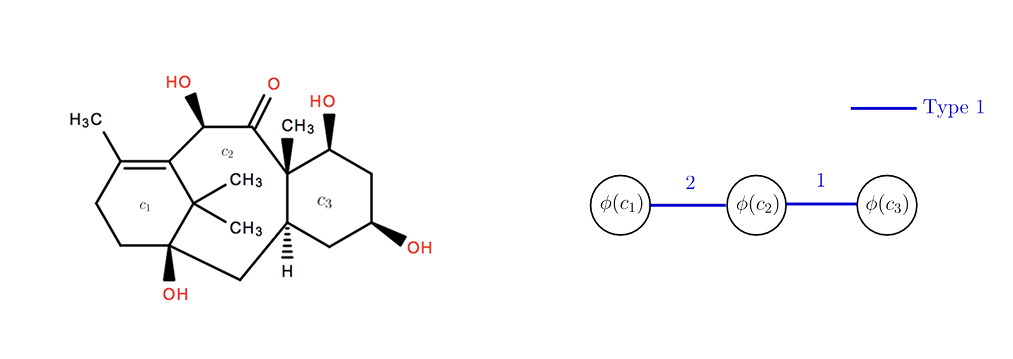
\includegraphics[scale=0.85]{type1_exemple.png}
\end{center}
\caption{Graphe moléculaire et graphe de cycles }
\end{figure}

\end{exemple}

\subsection{Le type 2 : Cycles indirectement liés}

Deux cycles sont indirectement liés lorsqu'ils sont reliés dans le graphe moléculaire par des chaînes. Dans la Figure \ref{grapheintuitif}, on a constaté qu'il fallait des informations supplémentaires pour décrire en la partie strcutrelle de la molécule.


Bien que les cycles $c_2$ et $c_3$ de la Figure \ref{type2} ne partagent pas d'atomes, une arête entre ces deux cycles dans $GC$ permettrait de lever l'ambiguïté.

Soit un graphe de cycles $GC$ et deux cycles $c_1, c_2 \in VC$. Les fonctions d'étiquettages des arêtes sont telles que:

\begin{itemize}
\item $\varphi([c_1,c_2]) = 2 $ si l'arête est de type $2$. C'est à dire qu'il existe dans $G$ une chaîne d'atomes ne passant par aucun cycle de $VC$ reliant les cycles $c_1$ et $c_2$,
\item $\chi([c_1,c_2]) $ pour une arête de type $2$ est égale à la longueur de la plus petite chaîne reliant $c_1$ et $c_2$ dans $G$.
\end{itemize} 

\begin{exemple} Les cycles élémentaires $c_2$ et $c_3$ appartiennent à deux composantes $2-$connexes différentes. La plus petite chaîne relaint ces $é$ cycles est de longueur $2$.

\begin{figure}[H]
\label{type2}

\begin{center}
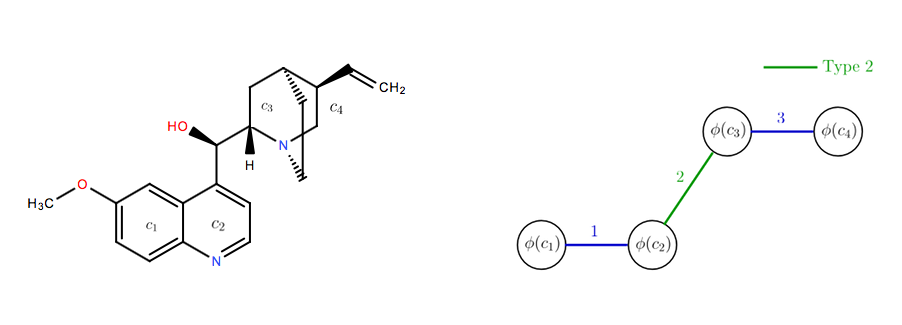
\includegraphics[scale=0.45]{type2_exemple.png}
\end{center}
\caption{Graphe moléculaire et graphe de cycles }
\end{figure}

\end{exemple}

Maintenant que nous avons défini les types d'interconnexions, nous allons procédér au choix de la base de cycles pour construire le graphe de cycles.

\section{ Le générateur pour le graphe de cycles}
\label{generateurcycles}


On rappelle que l'on souhaite avoir une représentation canonique de la partie structurelle de la molécule. Dans cette section, nous allons construire l'ensemble de sommets $VC$ et définir la fonction $\phi(VC)$. 

\subsection{Une base de cycles comme générateur ?}


Une base de cycles de longueur minimum est un candidat potentiel pour construire le graphe de cycles. Il contient un nombre fini de cycles et toutes les bases de cycles d'un graphe ont le même nombre de cycles.

En reprenant le graphe moléculaire de la quinine, on constate dans la Figure \ref{lesbases} que ce graphe possède $3$ bases de cycles différentes. Deux cycles de l'ensemble $\{c_3, c_4, c_5\}$ suffisent pour obtenir une base.

\begin{figure}[H]
\label{lesbases}

\begin{center}
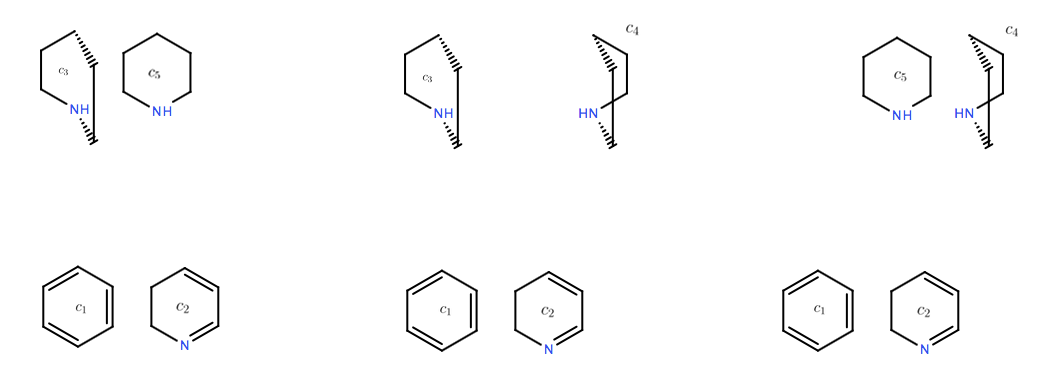
\includegraphics[scale=0.75]{base_complete.png}
\end{center}
\caption{Les bases de cycles pour le graphe moléculaire de la quinine}
\end{figure}

En construisant les graphes de cycles avec chacune de ces bases on obtient respectivement $GC_1$,$GC_2$ et $GC_3$. Les graphes $GC_2$ et $GC_3$ sont isomorphes. Le choix d'une base de cycle pourrait donner un graphe de cycles différent pour une même molécule.


\begin{figure}[H]
\label{bases}

\begin{center}
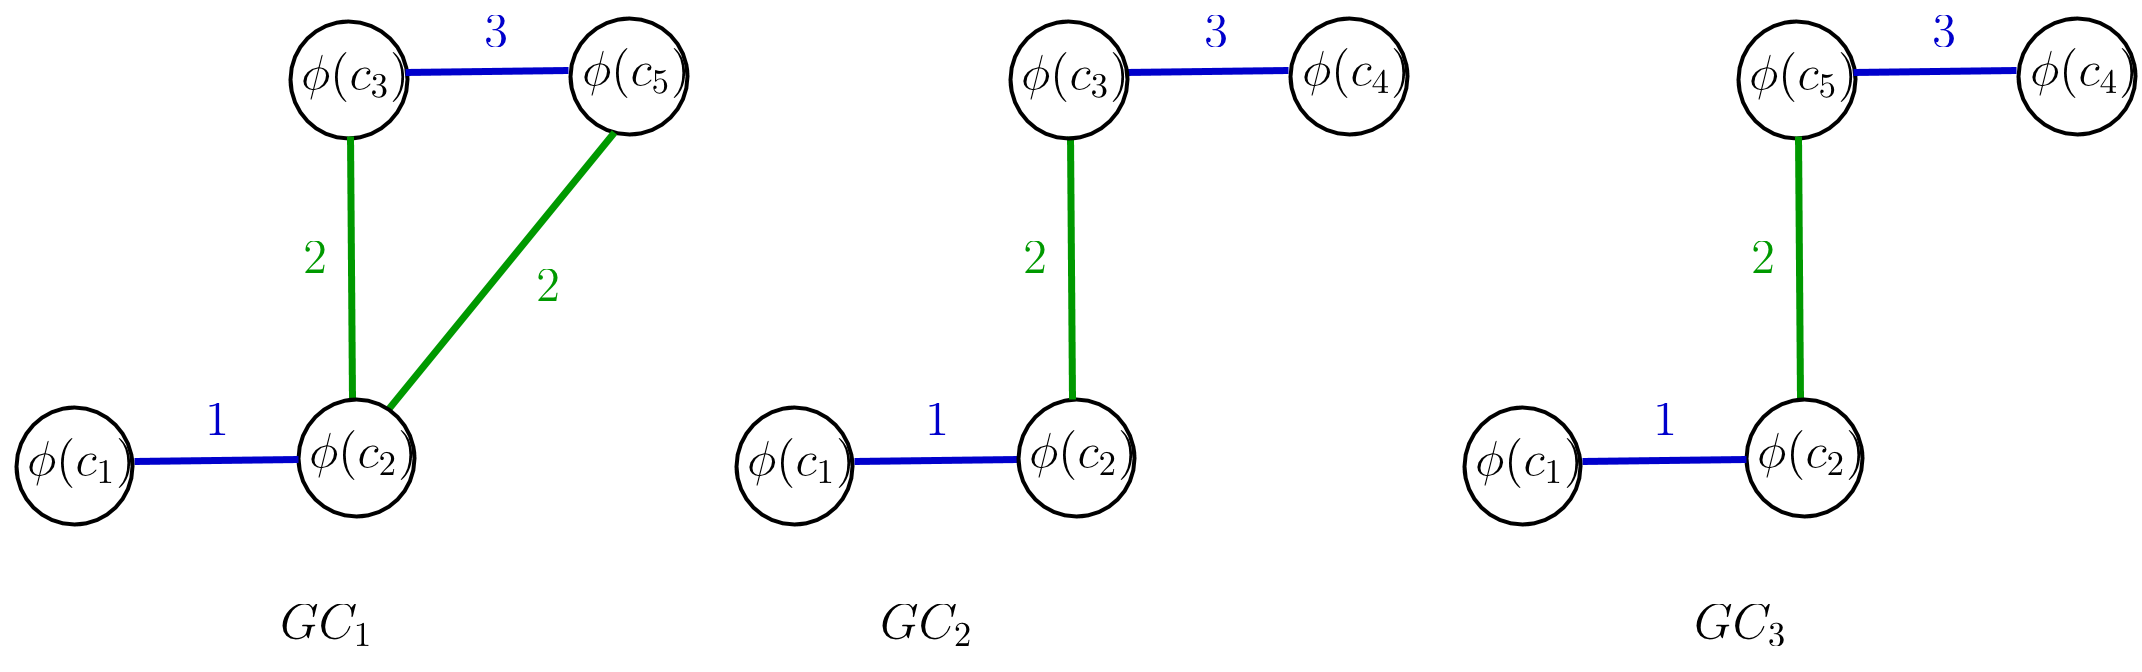
\includegraphics[scale=0.35]{graphes_base.png}
\end{center}

\caption{Les graphes de cycles pour les différentes bases de cycles.}
\end{figure}
Dans ce cas, si on prend deux fois la même molécule et deux bases de cycles différentes, la mesure de similarité concluerait que les graphes de cycles ne sont pas totalement similaires. 


Cela deviendrait encore plus ambigüe s'il existe des cycles raccrochés au composé xxxx (voir Figure \ref{differentsgraphes}). Si on continue d'étendre ce graphe moléculaire, les graphes de cycles d'une molécule pourraient prêter à confusion pour la similarité. 

\begin{figure}[H]
\label{differentsgraphes}
\begin{center}
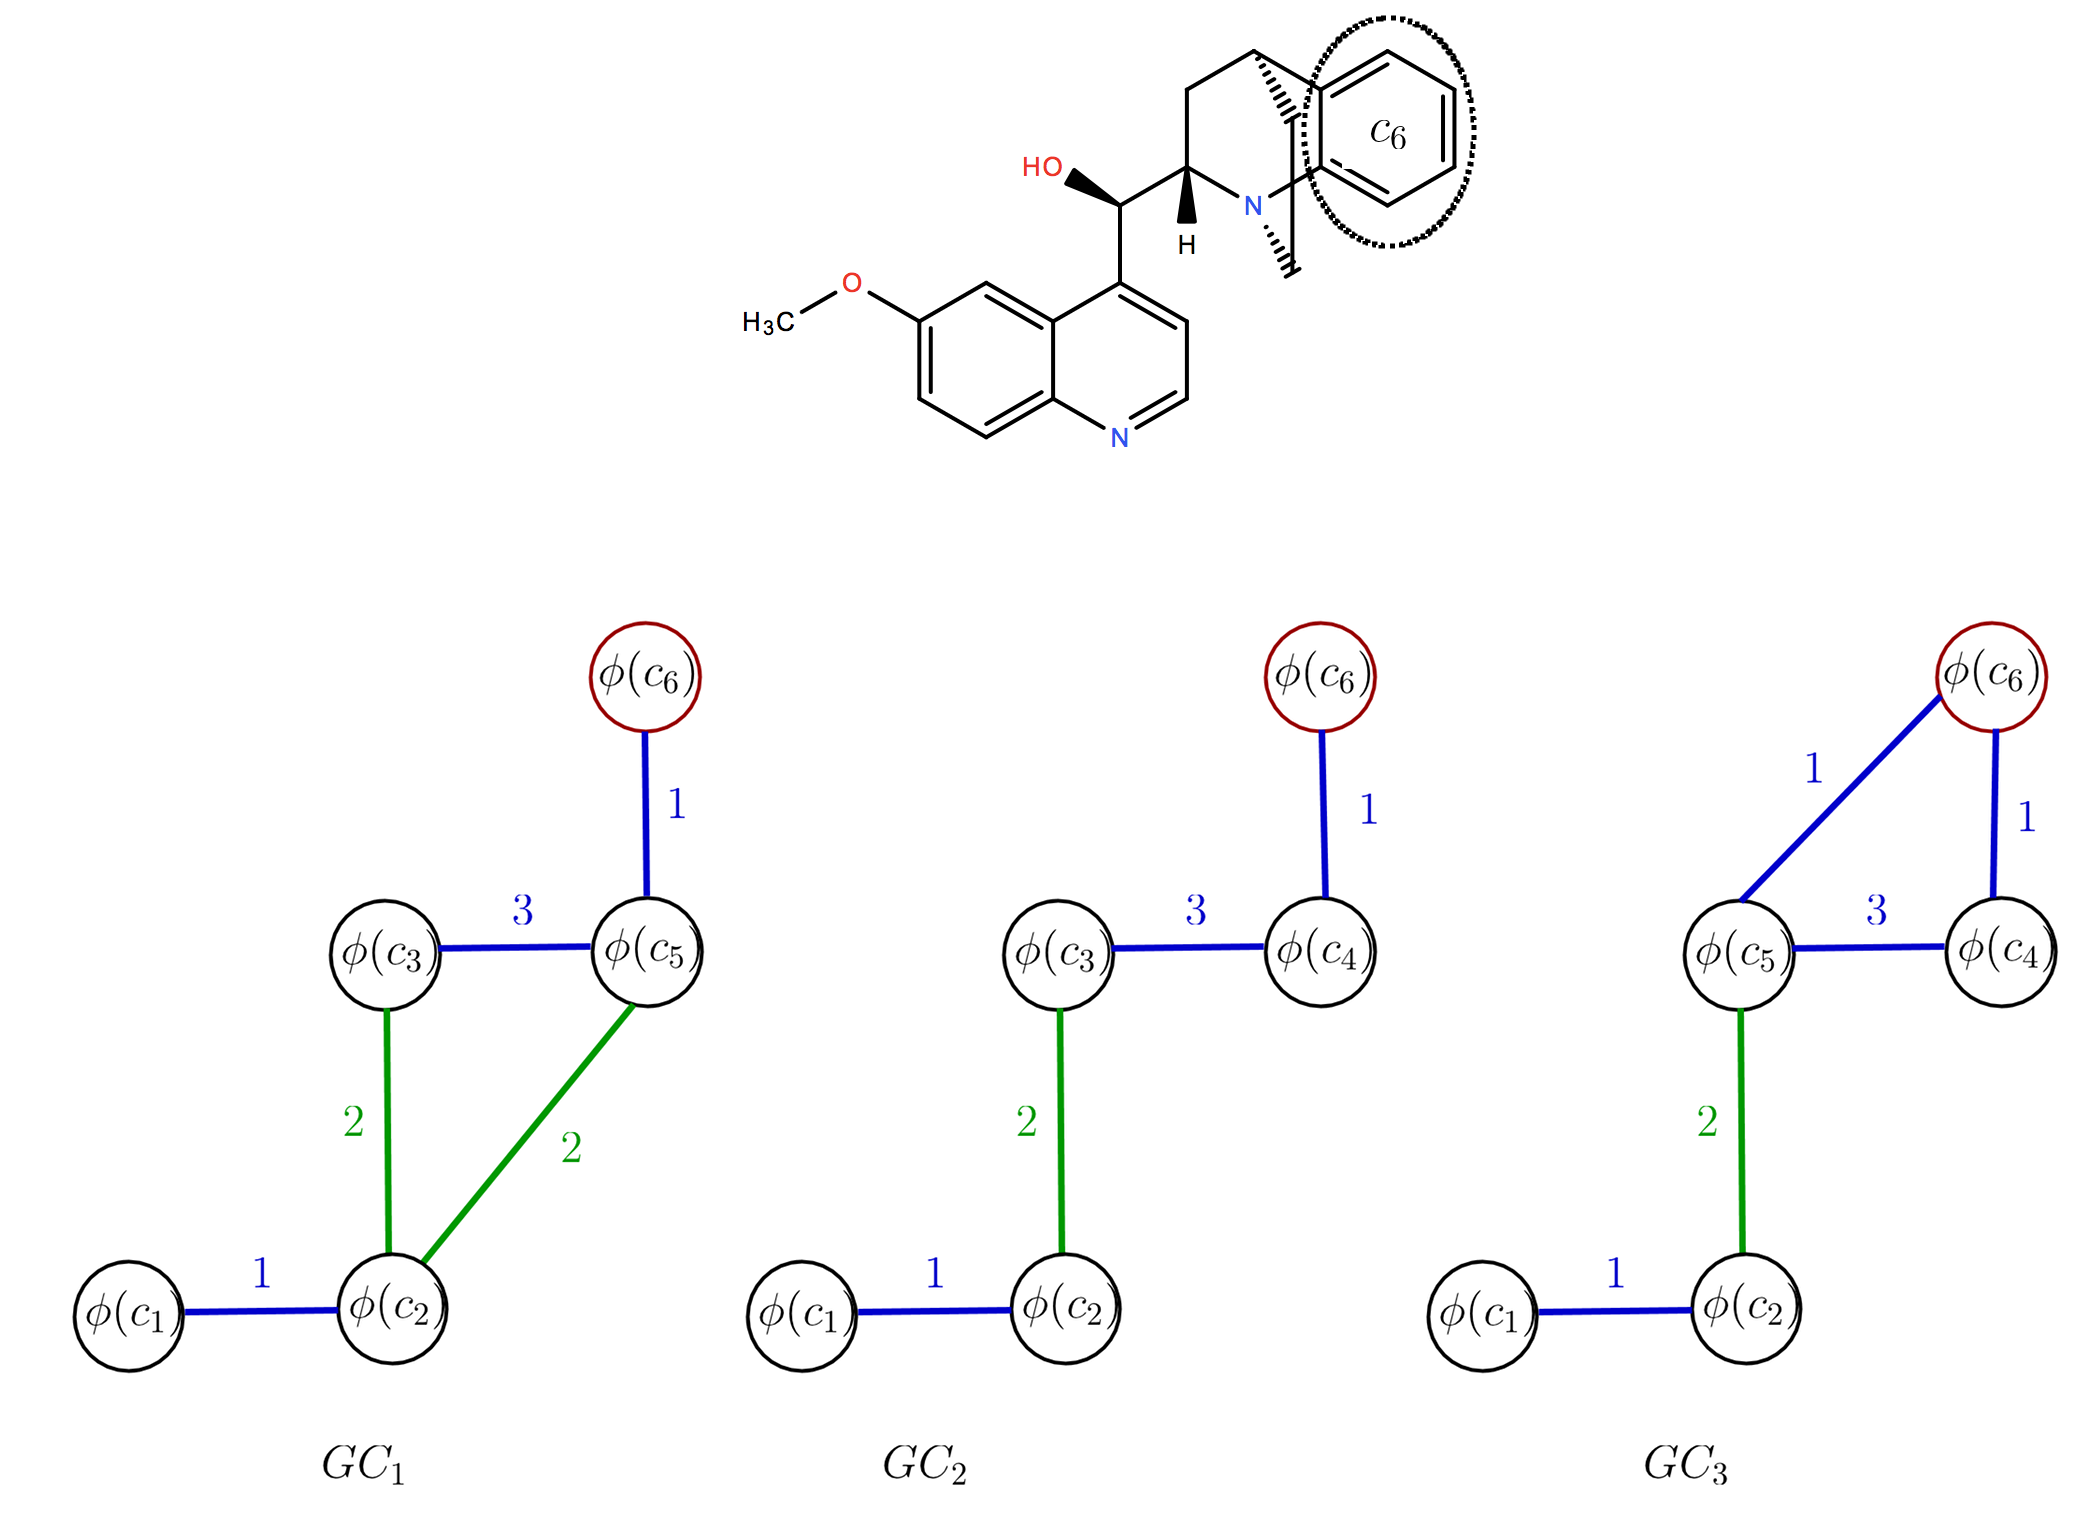
\includegraphics[scale=0.4]{graphes_different.png}
\end{center}
\caption{L'ajout d'un cycle dans un graphe moléculaire augmente potentiellemnt le nombre de graphes de cycles possibles.}
\end{figure}

En observant l'algorithme de Horton, précisement au niveau de la selection des cycles indépendants, deux des cycles $c_3, c_4$ et $c_5$ seront selectionnés en fonction de l'ordre de classement qui n'est pas prédefini.


%\subsection{Générateur canonique}

Pour construire un générateur canonique pour le graphe de cycles, nous utilisons l'algorithme de Horton et l'algorithme de McKay.  La première étape consiste à numéroter canoniquement les sommets du graphe moléculaire en utilisant l'algorithme d'isomorphisme de McKay. Ensuite, cette numérotation de sommets est utilisée pour obtenir une base de cycle de longueur minimum $\mathcal{B}$ avec l'algorithme de Horton. Et finalement, on rajoute eventuellement des cycles pour garantir la canonicité.

\subsection{Algorithme de McKay pour la numérotation canonique}

Cet algorithme a été conçu pour résoudre le problème d'isomorphisme de graphes. Décider de l'existence d’un isomorphisme entre deux graphes $G_1$ et $G_2$ est dans NP. L'algorithme de Brendan McKay \cite{Hartke} cherche un étiquetage canonique des sommets d'un graphe permettant leur ordonnancement. Si deux graphes possèdent le même étiquetage alors ils sont isomorphes \cite{McKay201494}. 

Cependant le problème peut être résolu en temps polynomial pour certaines classes de graphes, par exemple les graphes planaires ou les graphes de degré borné et en temps quasi-polynomial pour le cas général. Les graphes moléculaires se retrouvent dans cette catégorie car le degré des sommets est borné par le nombre de liaisons covalentes des atomes.

\begin{definition}
Une partition d'un ensemble $E$ est une collection d'ensembles disjoints deux à deux et non vides (appelées blocs dans la suite) dont l'union est $E$. Une partition ordonnée de $E$ est une partition dont on a ordonné les blocs. Lorsque chaque bloc d'une partition est de taille $1$, la partition est dite discrète. 
\end{definition}

L'algorithme de McKay commence par établir un partitionnement ordoné et équitable des sommets en fonction du degré. Une partition dans lequel les sommets du même bloc sont deux à deux adjacents à un nombre identique de sommets dans un autre bloc est une partition \textbf{équitable}. Avec une partition équitable, l'algorithme introduit des distinctions supplementaires entre les sommets. A chaque étape, il examine tous les choix pertinents en explorant systématiquement l’espace des partitions ordonnées équitables à l’aide d’un arbre de recherche. L'algorithme s'arrête lorsque chaque partition est discrète. 


Ensuite à chaque noeud final de l'arbre est une partition ordonée et discrète.  Chacune de ces partitions définit une nouvelle numérotation des sommets de $V$. La numeérotation se fait dans l'ordre dans lequel les sommets apparaisssent. %l'algorithme associe une permutation d'indices dans le graphe c'est à dire une nouvelle numérotation.

Chaque isomorphisme peut-être vu comme un mot en concatenant les ensembles de la partition.
\textcolor{red}{La numerotation canonique est l'isomorphisme ayant le mot le plus petit.pas tout a fait ! c'est un mot binaire, j'ecrirais la version exacte plus tard... DOIS JE RAJOUTER UN PETIT EXEMPLE POUR MONTRER COMMENT CA FONCTIONNNE ? } 

Cet algorithme est implémenté dans le package \textit{nauty}\cite{McKay201494} disponible sous differents systèmes d'exploitations (Windows, Mac OS, GNU/Linux).


\subsection{Algorithme de Horton pour une base de cycles}

Cet algorithme calcule une base de cycles de longueur minimum dans un graphe. Soit un graphe $G = (V,E)$, l'algorithme de Horton\cite{horton} est polynomial en $\mathcal{O} (|E|^3\times |V|)$.


Il se base sur le théorème suivant : 

\begin{theorem}
Soit un sommet $v$ appartenant à un cycle $c$ dans une base de cycles de longueur minimum $\mathcal{B}$. Alors il existe une arête $(x,y)$ dans $c$ tel que : $c = P(v,x) + P(v,y) + (x,y)$ avec $P(v,x)$ un plus court chemin entre $v$ et $x$ dans $G$.
\end{theorem}

La première étape de l'algorithme consiste à trouver s'il existe, un plus court chemin entre chaque paire de sommet. Ensuite, on verifie s'il existe des cycles élémentaires entre chaque sommet et chaque arête du graphe. Cela permet d'obtenir au maximum $|E| \times |V|$ cycles élémentaires. À l'étape $3$, les cycles sont classés par taille croissante de manière à les selectionner dans cet ordre durant la dernière étape.

\vspace{0.5cm}
\begin{algorithm}[H]
\SetAlgoLined
\KwData{Un graphe simple $G=(V,E)$}
 \KwResult{Une base de cycles de longueur minimum $\mathcal{B}$}
Trouver un plus court chemin entre chaque paire de sommets de $V$ \;
Pour chaque sommet $v$ et chaque arête $(x,y)$ du graphe $G$, créer un cycle $c(v,x,y) = P(v,x) + P(v,y) + (x,y)$\;
Ordonner les cycles par taille croissant\;
Utiliser un algorithme glouton pour extraire une base de cycles de longueur minimum à partir des cycles obtenus\;
\caption{Algorithme de Horton}
\end{algorithm} 

\vspace{0.5cm}

L'étape $4$ consiste former une matrice binaire dans laquelle chaque ligne est un cycle (en respectant l'ordre effectué à l'étape $3$). Chaque colonne représente une arête du graphe. Si une arête appartient à un cycle la case associé aura la valeur $1$ et la valeur $0
$ sinon. L'élimination de Gauss peut alors être appliquée pour obtenir une base de cycle de longueur minimum.

\textcolor{red}{Un exemple?}


\subsection{Générateur canonique}

Pour obtenir le générateur canonique $\zeta$ d'un graphe moléculaire, on calcule une base de cycles de longueur minimum $\mathcal{B}$ en ayant au préalable effectué une numérotation canonique des sommets.
Ensuite pour résoudre le prolème engendré par la chiralité, on rajoute éventuellement à $\mathcal{B}$ l'intégralité des cycles respectant la règle suivante :

\begin{center}
$\forall c,c' \in \mathcal{B}$ on calcule $c" = c \oplus c'$ en combinant $c$ et $c'$. Si $c"$ est un cycle élementaire de taille plus petite ou égale à ceux de $c$ et $c'$ alors il pertinent pour le graphe de cycles.
\end{center}

La fonction d'etiquettage des sommets $\phi$ associe à chaque cycle, sa taille c'est dire le nombre d'atomes qu'il contient dans le graphe moléculaire.

Dans la figure \ref{graphequinine}, le graphe de cycles de la quinine conserve alors les trois cycles du composé chiral. Ces cycles partagent alors des arêtes de type $1$ avec $\phi(c_i)$ , la taille du cycle $c_i$.

\begin{figure}[H]
\label{graphequinine}
\begin{center}
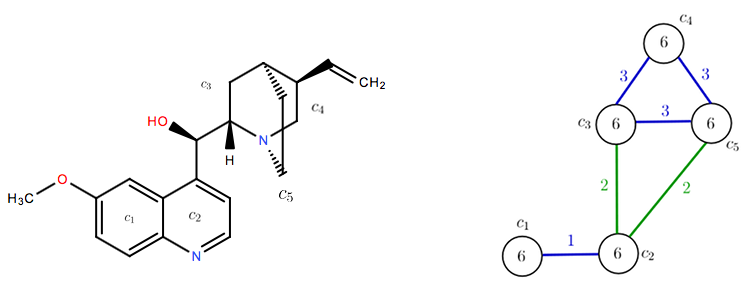
\includegraphics[scale=0.45]{graphe_quinine.png}
\end{center}
\caption{Le graphe de cycles $GC$ de la quinine.}
\end{figure}

La complexité de l'algorithme qui calcule le graphe de cycles d'un graphe $G$ est $\mathcal{O}(n^2.m^3)$.


\subsection{Générateur j-hierarchique }

Nous allons introduire la notion de $j-$hierarchique avec l'exemple suivant:

\begin{exemple}
On considère deux molécules struturellement similaires : la Strychnine et la Vomicine. Sur la figure \ref{hierarchiqueexemple}, si on prend en compte tous les cycles du générateur canonique, alors on trouverait que les graphes de cycles associés à ces molécules ne sont pas assez similaires avec en mesurant la similarité. 

\begin{figure}[H]
\label{hierarchiqueexemple}
\begin{center}
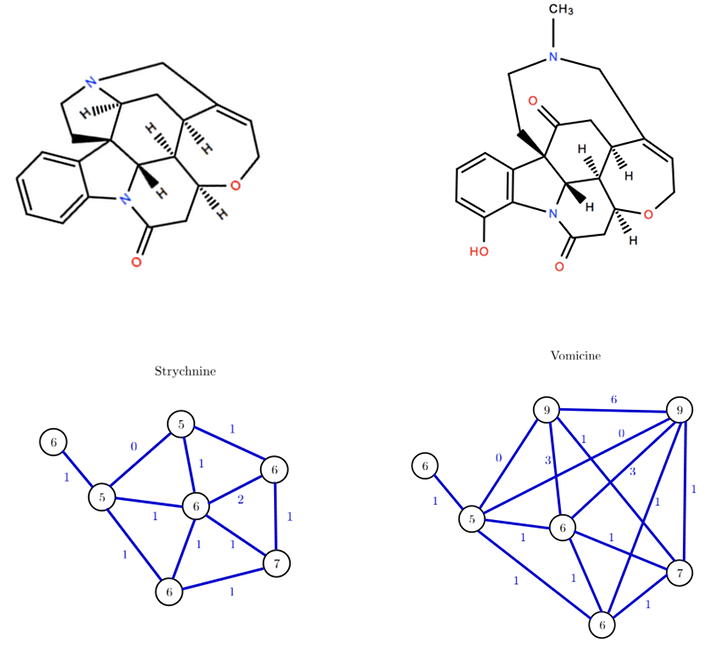
\includegraphics[scale=0.85]{j-hierarchique.png}
\end{center}
\caption{Les molécules : Strychnine et Vomicine avec leur graphe de cycles.}
\end{figure}
En effet, deux cycles de la Strychnine (de taille respectivent $5$ et $6$) ont fusionnés entraînant l'apparition de deux cycles de taille $9$ dans le graphe de cycles de la Vomicine. De plus, ces cycles ne sont pas chimiquement pertinents pour la Vomicine.

Si on reprend le générateur canonique de la Vomicine et on supprime les cycles de taille $9$, le nouveau graphe de cycles obtenu (dans la figure \ref{newjhierarchique}) capte mieux sa similarité avec la Strychnine.

\begin{figure}[H]
\label{newjhierarchique}
\begin{center}
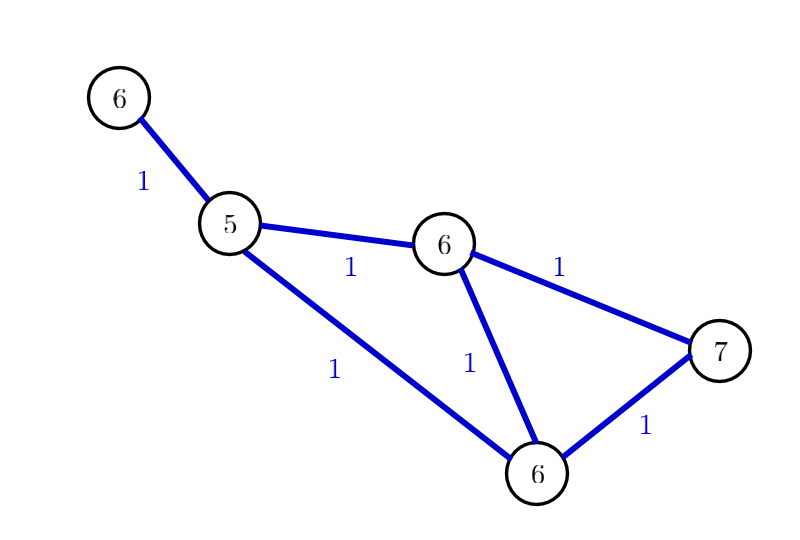
\includegraphics[scale=0.5]{gc_vomicine.png}
\end{center}
\caption{Le graphe de cycles de la Vomicine en supprimant les cycles de taille $9$.}
\end{figure}

%En effet, un cycle pertinent dans la Strychnine a été cassé pour obtenir la Vomicine. Cette modification de la structure de la Strychnine donne lieu à d'autres cycles plus grands et non pertinent pour la structure de la Vomicine.
\end{exemple}


\begin{definition}
Soit un générateur canonique $\zeta$ et un entier $j$. Le générateur $\zeta$ est $j-$hierarchique si le sous-ensemble contenant tous les cycles de $\zeta$ ayant une taille inférieure ou égale à $j$ génère tous les cycles de $G$ ayant une taille inférieure ou égale à $j$.
\end{definition}

Un générateur est \textit{hierarchique} si et seulement si il est $j-$hierarchique pour tout $j$. On note $\zeta_j$ le générateur $j-$hierarchique de $\zeta$. Le générateur canonique utilisé pour construire le graphe de cycles est hierarchique car la base de cycles de longueur minimum l'es.


\begin{lemme}
Toute base de cycles de longueur minimum d'un graphe est hierarchique.
\end{lemme}

\begin{preuve}
Soit $G$ un graphe et $\mathcal{B}$ une base de cycles de longueur minimum de $G$. $\forall j, \mathcal{B}_j$ est une base de cycles de longueur minimum pour les cycles de longueur inférieur ou égal $j$.

Supposons que $\mathcal{B}$ n'est pas hierarchique; Cela signifie qu'il existe un entier $j$ tel que $\mathcal{B}_j$ n'est pas $j-$hierarchique.

Soit un entier $j$ tel que $\mathcal{B}_j$ n'est pas $j-$hierarchique. Il existe par définition un cycle $c \notin \mathcal{B}$ tel que $|c| \leq j$ et $c$ ne peut-être généré en utilisant les cycles de $\mathcal{B}_j$. 

Prenons dans $\mathcal{B}$ un ensemble de cycles $\{c_1, c_2, ..., c_{\alpha}\}$ tel que $ c = c_1 \oplus c_2 \oplus ... \oplus c_{\alpha -1 } \oplus c_{\alpha}$. Supposons que $c_{\alpha}$ est un cycle de longueur maximum dans $\{c_1, c_2, ..., c_{\alpha}\}$. Puisque $c$ ne peut-être généré par $\mathcal{B}_j$ alors $|c_{\alpha}| > j$.

De plus, $\oplus$ est associatif et commutatif, on a $c_{\alpha} = c_1 \oplus c_2 \oplus ... \oplus c_{\alpha -1 }\oplus c$. Soit $\mathcal{B}' = \mathcal{B} \backslash \{c_{\alpha}\}\cup \{c\} $, $\mathcal{B}'$ est aussi une base de cycle.

La longueur de la base $\mathcal{B}'$ est $|\mathcal{B}'| = |\mathcal{B}| -|c_{\alpha}|+ | c| $, donc $|\mathcal{B}'| < |\mathcal{B}| $. Il y'a contradiction car $\mathcal{B}$ est une base de cycle de longueur minimum.
\end{preuve}


De facon générale, les cycles chimiquement pertinents pour la structure d'une molécule sont de taille inférieur ou égale à $8$.  Mais il arrive que des cycles très grands le sont dans certains graphes moléculaires. Dans la figure \ref{ampho}, l'Amphotéricin B possède un cycle de taille $36$ qui fait sa particularité.


\begin{figure}[H]
\label{ampho}
\begin{center}
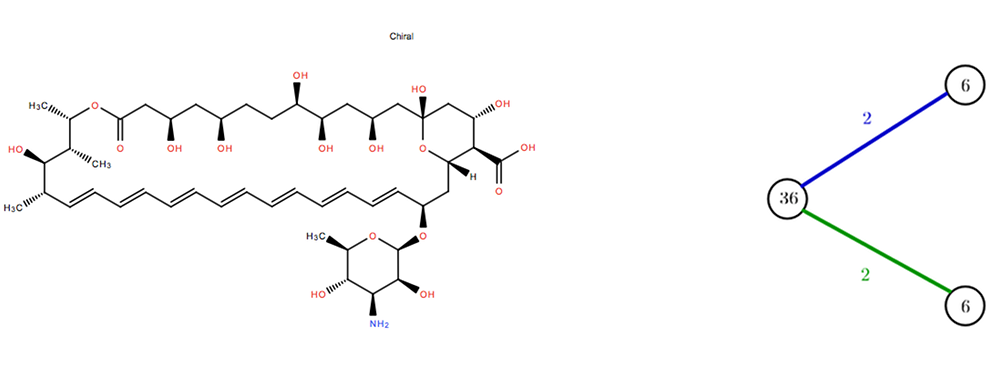
\includegraphics[scale=0.75]{amphotericin3.png}
\end{center}
\caption{Le graphe moleculaire et le graphe de cycles de l'Amphotéricin B.}
\end{figure}

\paragraph{} Dans ce chapitre, nous avons définit formellement le graphe de cycles. Pour le calculer, nous utilisons l'algorithme de McKay pour la numérotation canonique des sommets du graphe moléculaire et ensuite l'algorithme de Horton pour construire un générateur canonique. Par la suite, nous rajoutons éventuellement des cycles supplémentaires pour assurer la canonicité du graphe de cycles. Le choix du paramètre $j$ sera important pour mesurer la similarité dans le chapitre suivant et permet de valider le modèle de graphe de cycles.
\chapter{Évaluation de la similarité moléculaire}
\label{chap4}
\section{Titre de la premiere section}
Bla bla bla
\section{Titre de la seconde section}
Re-bla bla bla

\section{Conclusion}
Conclusion du chapitre.
\chapter{Similarité pour la catégorisation des réactions}
\label{chap5}
\section{Titre de la premiere section}
Bla bla bla
\section{Titre de la seconde section}
Re-bla bla bla

\section{Conclusion}
Conclusion du chapitre.
\chapter*{Conclusion}
Bla bla bla.
%\nocite{*}

\bibliography{biblio}

%\appendix
\backmatter
%\makeback
\end{document}